\documentclass{ximera}

\title[Breal-grond]{This is the sample! Waffle!  Iff!}

\newcommand{\mypreamble}{WHEEEEE}
%%% Local Variables:
%%% mode: latex
%%% TeX-master: t
%%% End:


\begin{document}
\begin{abstract}
  The begining and now an instructor! I am doing math like $\arcsin$. AGAIN
\end{abstract}

\maketitle

\mypreamble


I am testing the waffle and the iff statement.

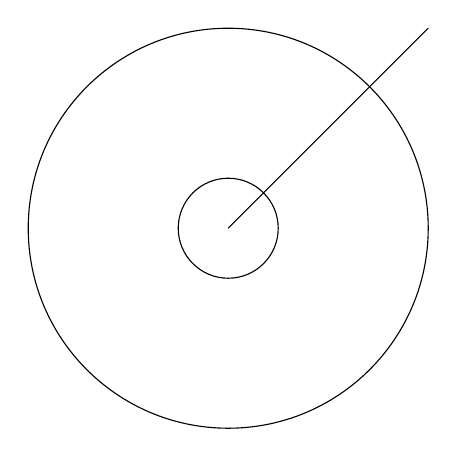
\begin{tikzpicture}
  \draw (0,0) circle (1in);
  \draw (0,0) circle (0.25in);
  \draw (0,0) -- (1in,1in);
\end{tikzpicture}

\youtube{eGXGlG5CuYE}

\end{document}

%%% Local Variables:
%%% mode: latex
%%% TeX-master: t
%%% End:
% Changed at Mon Jul 27 22:23:04 EDT 2015
% Changed at Mon Jul 27 22:24:20 EDT 2015
% Changed at Mon Jul 27 22:25:23 EDT 2015
% Changed at Mon Jul 27 22:30:13 EDT 2015
% Changed at Mon Jul 27 22:32:16 EDT 2015
% Changed at Mon Jul 27 22:33:48 EDT 2015
% Changed at Tue Jul 28 00:05:31 EDT 2015
% Changed at Tue Jul 28 00:05:33 EDT 2015
% Changed at Tue Jul 28 00:05:34 EDT 2015
% Changed at Tue Jul 28 00:05:35 EDT 2015
% Changed at Tue Jul 28 00:05:55 EDT 2015
% Changed at Tue Jul 28 00:05:56 EDT 2015
% Changed at Tue Jul 28 00:05:57 EDT 2015
% Changed at Tue Jul 28 00:05:58 EDT 2015
% Changed at Tue Jul 28 00:05:59 EDT 2015
% Changed at Tue Jul 28 00:06:00 EDT 2015
% Changed at Tue Jul 28 00:06:01 EDT 2015
% Changed at Tue Jul 28 00:06:03 EDT 2015
% Changed at Tue Jul 28 00:06:04 EDT 2015
% Changed at Tue Jul 28 00:06:28 EDT 2015
